
\newcommand\tfuzz[1]{{\scriptsize {\tt #1}}}

%----------------------------------------
\begin{frame}<0>
  \frametitle{ASCII representation} \small



\small
\centering
\begin{tabular}{lll}
$\neg$               & \ifuzz{not}     & \tfuzz{!}\\
$\lor$               & \ifuzz{or}      & \tfuzz{|}\\
$\wedge$             & \ifuzz{and}     & \tfuzz{\&}\\
$\next$              & \ifuzz{next}    & \tfuzz{()}\\
$\until$             & \ifuzz{until}   & \tfuzz{U}\\
$\prev$              & \ifuzz{prev}    & \tfuzz{(*)}\\
$\since$             & \ifuzz{since}   & \tfuzz{S}\\
$\Diamond$           & \ifuzz{eventually} & \tfuzz{<>}\\ 
$\Box$               & \ifuzz{always}  & \tfuzz{[]}\\
$\DDiamond$          & \ifuzz{once}    & \tfuzz{<*>}\\
$\BBox$              & \ifuzz{sofar}   & \tfuzz{[*]}\\
$\wuntil$            & \ifuzz{wuntil}  & \tfuzz{WU}\\
$\wsince$            & \ifuzz{wsince}  & \tfuzz{WS}\\
$\wnext$             & \ifuzz{wnext}   & \tfuzz{()?}\\
$\wprev$             & \ifuzz{wprev}   & \tfuzz{(*)?}\\
$\Sigma^{+}_{[a,b]}$ & \ifuzz{count (a,b)} & \tfuzz{@ (a,b)}\\
$\Sigma^{-}_{[a,b]}$ & \ifuzz{countpast (a,b)} & \tfuzz{@* (a,b)}\\
$\Sigma^{+}_{a}$     & \ifuzz{count a} & \tfuzz{@ a}\\
$\Sigma^{-}_{a}$     & \ifuzz{countpast a} & \tfuzz{@* a}\\
$\Next_n$            & \ifuzz{next n}  & \tfuzz{()} n\\
$\prev_n$            & \ifuzz{prev n}  & \tfuzz{(*) n}
\end{tabular}

\end{frame}

%----------------------------------------
\begin{frame}
  \frametitle{Rover example} \small

\begin{figure}
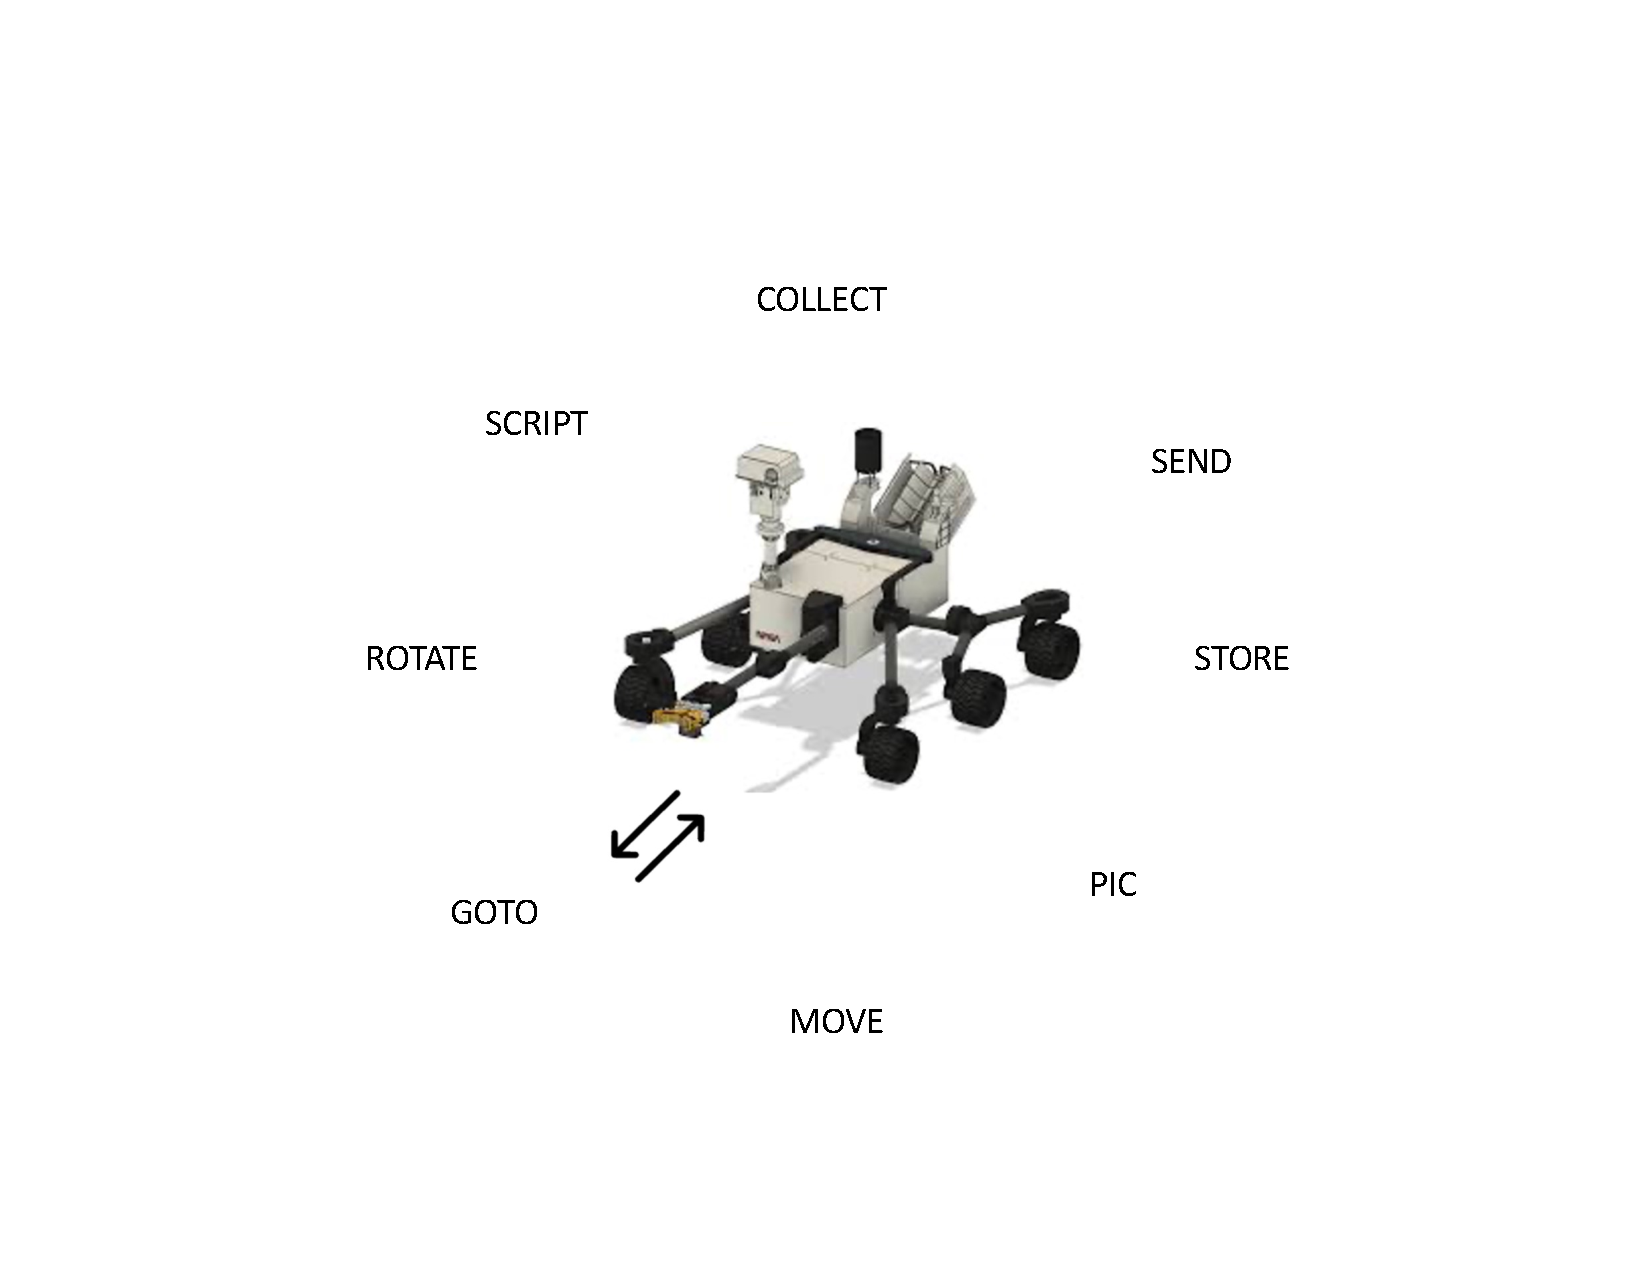
\includegraphics[width=1.0\textwidth]{figures/rover-actions.pdf}
%\caption{Your caption}
\end{figure}

\end{frame}


%----------------------------------------
\begin{frame}
  \frametitle{Rover example - commands} \small

{\scriptsize
\begin{center}
\texttt{direction} = \{ \texttt{forward},\ \texttt{backward} \} \\[0.5ex]
\texttt{image\_quality} = \{ \texttt{low},\ \texttt{medium},\ \texttt{high} \}
\end{center}
}

{\scriptsize
\[
\begin{array}{l}
\texttt{ROTATE}(number\!:\!\texttt{uint},\ time\!:\!\texttt{uint},\ angle\!:\!\texttt{float}) \\
\quad \text{where } -180 \le \texttt{angle} \le 180 \\ \\[0.5ex]
%
\texttt{GOTO}(number\!:\!\texttt{uint},\ time\!:\!\texttt{uint},\ x\!:\!\texttt{float},\ y\!:\!\texttt{float}) \\
\quad \text{where } -10000 \le \texttt{x,y} \le 10000 \\ \\[0.5ex]
%
\texttt{MOVE}(number\!:\!\texttt{uint},\ time\!:\!\texttt{uint},\ dir\!:\!\texttt{direction},\ distance\!:\!\texttt{float}) \\
\quad \text{where } 1 \le \texttt{distance} \le 1000 \\ \\[0.5ex]
%
\texttt{PIC}(number\!:\!\texttt{uint},\ time\!:\!\texttt{uint},\ quality\!:\!\texttt{image\_quality},\ images\!:\!\texttt{uint}) \\
\quad \text{where } 1 \le \texttt{images} \le 10 \\ \\[0.5ex]
%
\texttt{STORE}(number\!:\!\texttt{uint},\ time\!:\!\texttt{uint},\ file\!:\!\texttt{string},\ images\!:\!\texttt{uint}) \\
\quad \text{where } 1 \le \texttt{images} \le 10 \\ \\[0.5ex]
%
\texttt{SEND}(number\!:\!\texttt{uint},\ time\!:\!\texttt{uint},\ file\!:\!\texttt{string}) \\ \\[0.5ex]
%
\texttt{COLLECT}(number\!:\!\texttt{uint},\ time\!:\!\texttt{uint},\ file\!:\!\texttt{string},\ sample\!:\!\texttt{string}) \\ \\[0.5ex]
%
\texttt{SCRIPT}(number\!:\!\texttt{uint},\ time\!:\!\texttt{uint},\ script\!:\!\texttt{string},\ file\!:\!\texttt{string}) \\[0.5ex]
\end{array}
\]
}

\end{frame}

%----------------------------------------
\begin{frame}
  \frametitle{XML representation of commands} \scriptsize

\begin{figure}
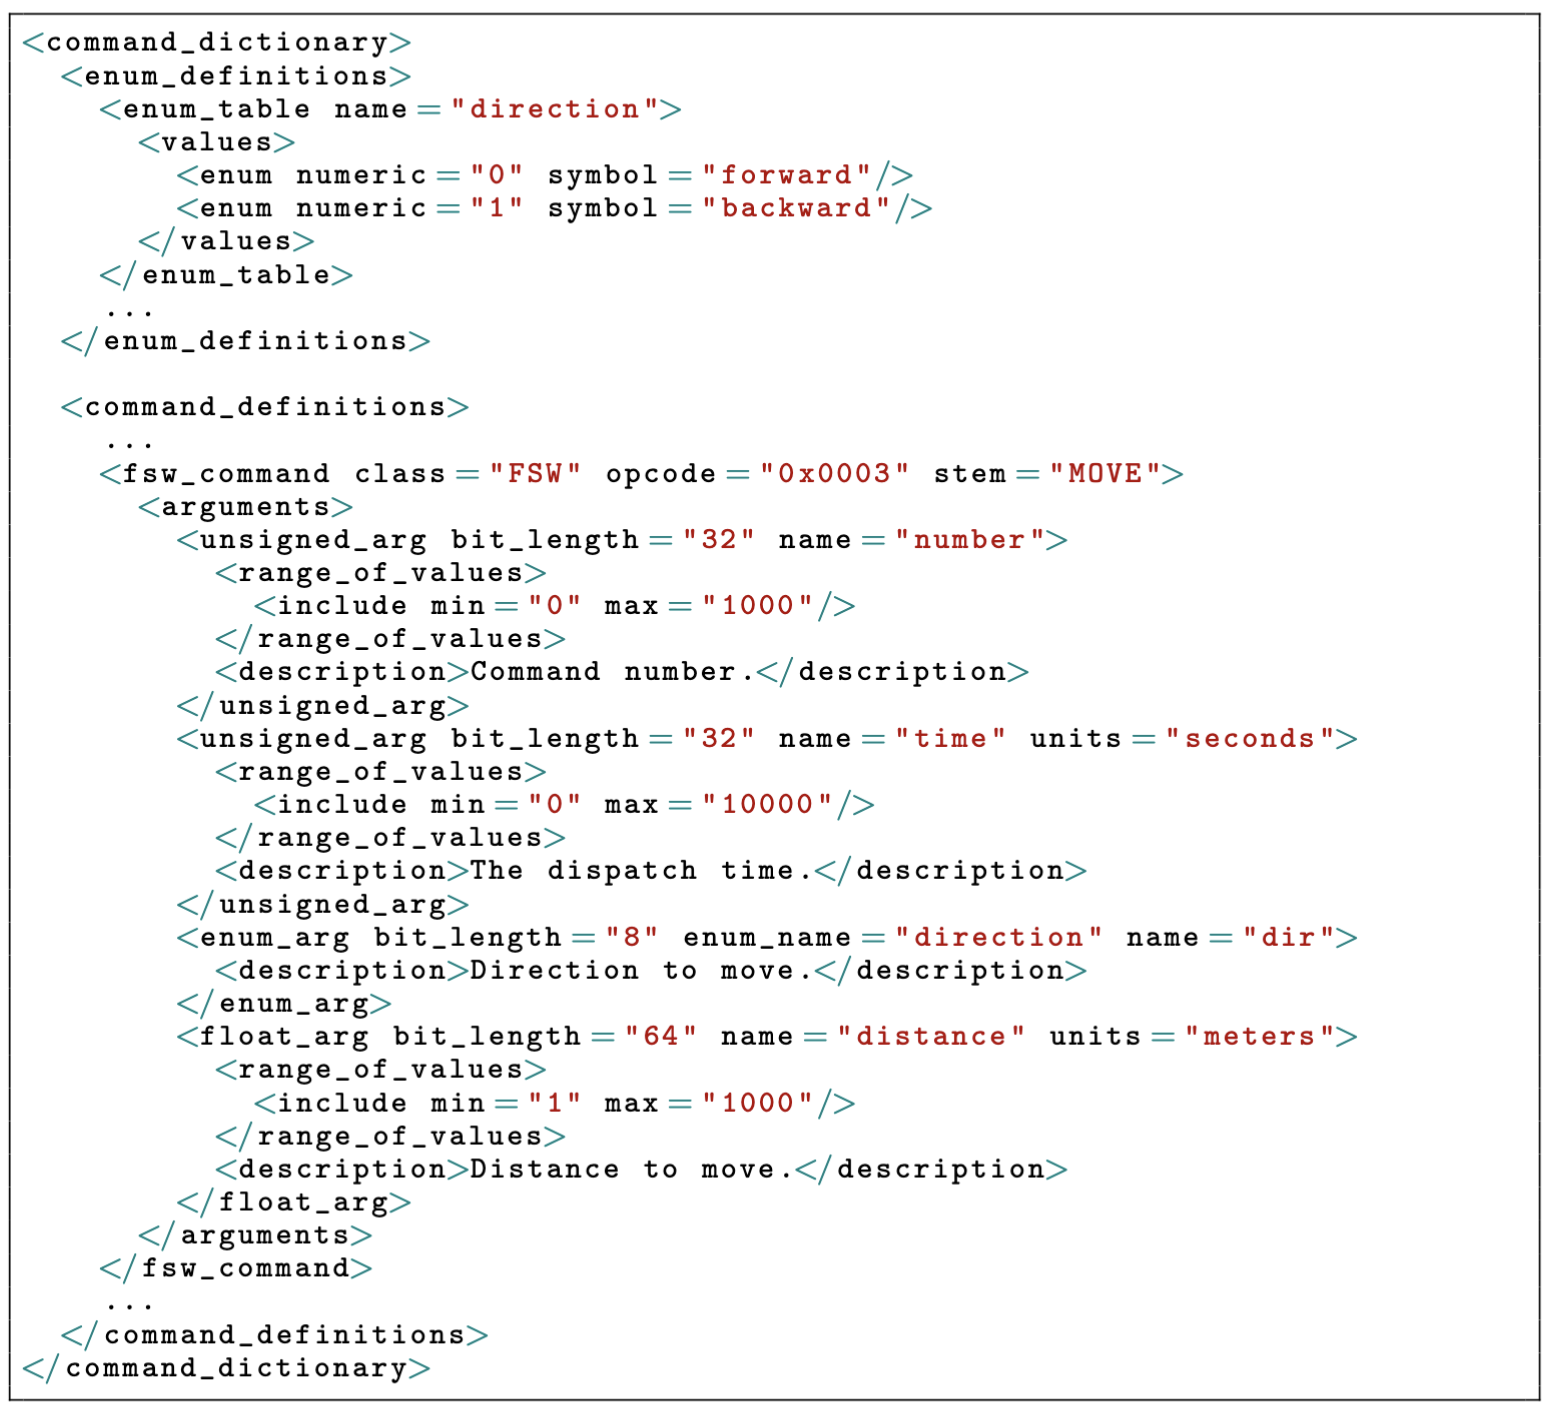
\includegraphics[width=0.71\textwidth]{figures/xml-commands.png}
%\caption{Your caption}
\end{figure}

\end{frame}


%----------------------------------------
\begin{frame}[fragile]
  \frametitle{Activating fuzz in Python} \small

% Types

% \begin{lstlisting}[language=python,frame=single]
% Command = Dict[str, Union[int, float, str]]
% Test = list[Command]

% \end{lstlisting}

% \pause

API

\begin{lstlisting}[language=python,frame=single]
def generate_tests(spec: Optional[str] = None, 
                   test_suite_size: Optional[int] = None, 
                   test_size: Optional[int] = None) -> list[Test]:
\end{lstlisting}

%\pause

% Configuration file used for default values

% \begin{lstlisting}[language=json]
% {
%     "cmd_files": ["xml/rover_commands.xml"],
%     "spec_file": "spec.txt",
%     "test_suite_size": 10,
%     "test_size": 10
% }
% \end{lstlisting}

\end{frame}

%----------------------------------------
\begin{frame}[fragile]
  \frametitle{Call fuzz without any constraints} \small

\begin{lstlisting}[language=python,frame=single]
from fuzz import generate_tests

tests = generate_tests(spec='', test_suite_size=100, test_size=10)
for test in tests:
    for cmd in test:
        print(cmd)
\end{lstlisting}

\pause

Yields a test of unconstrained random commands

\begin{lstlisting}[language=python,frame=single]
{'name': 'ROTATE', 'number': 51, 'time': 944, 'angle': -150.42}
{'name': 'SCRIPT', 'number': 75, 'time': 287, 'script': '...', 'file': '...'}
{'name': 'PIC', 'number': 64, 'time': 491, 'quality': 'low', 'images': 8}
{'name': 'SCRIPT', 'number': 48, 'time': 598, 'script': '...', 'file': '...'}
{'name': 'COLLECT', 'number': 39, 'time': 583, 'file': '...','sample': '...'}
{'name': 'COLLECT', 'number': 89, 'time': 78, 'file': '...', 'sample': '...'}
{'name': 'ROTATE', 'number': 87, 'time': 28, 'angle': 76.22}
{'name': 'GOTO', 'number': 90, 'time': 2, 'x': -8132.07, 'y': 4708.92}
{'name': 'PIC', 'number': 58, 'time': 531, 'quality': 'high', 'images': 6}
{'name': 'STORE', 'number': 74, 'time': 981, 'file': '...', 'images': 3}  
\end{lstlisting}

\end{frame}


%----------------------------------------
\begin{frame}[fragile]
  \frametitle{Defining constraints on all (any) commands} \small

\begin{block}{Requirements}
\begin{enumerate}
    \item Time must progress with steps no less than 10.
    \item Command numbers must increase by 1.
\end{enumerate}
\end{block}

\begin{lstlisting}[language=fuzzdsl,frame=single]
  rule p1: 
    always [any(time=t1?)] wnext [any(time=t2?)] t2 >= t1 + 10

  rule p2: 
    any(number=1) 
    and
    always [any(number=n1?)] wnext [any(number=n2?)] n2 = n1 + 1
\end{lstlisting}

\end{frame}


%----------------------------------------
\begin{frame}[fragile]
  \frametitle{Defining constraints on command arguments} \small

\begin{block}{Requirements}
\begin{enumerate}
    \setcounter{enumi}{2}
    \item The angle argument to ROTATE must be between -90 and 90.
    \item The distance argument to MOVE must be 1, 2 or 3.
\end{enumerate}
\end{block}

\begin{lstlisting}[language=fuzzdsl,frame=single]
  rule p3:   
    always [ROTATE(angle=a?)] -90 <= a <= 90
    
  rule p4: 
    always [MOVE(distance=d?)] (d = 1 or d = 2 or d = 3)   
\end{lstlisting}

\end{frame}


%----------------------------------------
\begin{frame}[fragile]
  \frametitle{Defining constraints on the future} \small

\begin{block}{Requirements}
\begin{enumerate}
\setcounter{enumi}{4}
\item  A MOVE command going backward, with a distance 'd', must be later followed be a ROTATE command, 
rotating with an angle 'a' satisfying $(d \le 1 \wedge a = 45) \vee (d > 1 \wedge a = 20)$.
\item Every GOTO command must be followed only by GOTO commands that move ``northeast'' (increasing in both x and y).
\end{enumerate}
\end{block}

\begin{lstlisting}[language=fuzzdsl,frame=single]
  rule p5: 
    always [MOVE(dir=direction.backwards,distance=d?)] 
      eventually <<ROTATE(angle=a?)>> 
                     ((d <= 1 and a = 45) or (d > 1 and a = 20))

  rule p6: 
    always [GOTO(x=x1?,y=y1?)] 
      always [GOTO(x=x2?,y=y2?)]  
        (x2 > x1 and y2 > y1)    
\end{lstlisting}

\end{frame}


%----------------------------------------
\begin{frame}[fragile]
  \frametitle{Defining constraints on strings with regular expressions} \small

\begin{block}{Requirements}
\begin{enumerate}
\setcounter{enumi}{6}
\item  if '$i$' high quality images are taken, then eventually a subset '$j$' ($0 < j \le i$)
of those images must be stored in a file with a name matching the regular
expression \verb+\d\d\d.img+ (e.g. {\tt 134.img}), and after that, this file must be sent to
the orbiting satellite.
\end{enumerate}
\end{block}

\begin{lstlisting}[language=fuzzdsl,frame=single]
  rule p7: 
    always [PIC(quality=image_quality.high, images=i?)]
      eventually <<STORE(file=f?, images=j?)>>
        (
          f |- /\d\d\d\.img/ 
          and
          0 < j <= i 
          and
          eventually SEND(file=f)
        ) 
\end{lstlisting}

\end{frame}


%----------------------------------------
\begin{frame}[fragile]
  \frametitle{Defining constraints about the past} \small

\begin{block}{Requirements}
\begin{enumerate}
\setcounter{enumi}{7}
\item If '$j$' images are stored in a file, then  
this file must not have been stored before, and also there must
have been taken a high quality picture in the past of a number of images '$i$'
($i \ge j$), and no file is stored since then except the current one.
\end{enumerate}
\end{block}

\begin{lstlisting}[language=fuzzdsl,frame=single]
  rule p8: 
    always [STORE(file=f?,images=j?)]
        prev ( 
          not once STORE(file=f) 
          and 
          (
            not STORE() 
            since 
            <<PIC(images=i?, quality=image_quality.high)>> i >= j
          )
        ) 
\end{lstlisting}

\end{frame}


%----------------------------------------
\begin{frame}[fragile]
  \frametitle{Defining constraints applying operations to data} \small

\begin{block}{Requirements}
\begin{enumerate}
\setcounter{enumi}{8}
\item If a sample collection named '$s$' is collected and the analysis result is stored in a
file '$f$', then later, without any other collection in
between, a script execution is commanded on that file '$f$',
where the script is named by concatenating \verb+"run_"+ with the sample name '$s$' 
and then \verb+".py"+.
\end{enumerate}
\end{block}

\begin{lstlisting}[language=fuzzdsl,frame=single]
  rule p9:     
    always [COLLECT(file=f?, sample=s?)] 
     next (
       not COLLECT()  
       until <<SCRIPT(script = k?, file=f)>> k = "run_" + s + ".py"
     )  
\end{lstlisting}

\end{frame}


%----------------------------------------
\begin{frame}[fragile]
  \frametitle{Defining constraints forcing commands to occur} \small

\begin{block}{Requirements}
\begin{enumerate}
\setcounter{enumi}{9}
\item We want to see a MOVE, a PIC with high image quality, 
and a COLLECT command.
\end{enumerate}
\end{block}

\begin{lstlisting}[language=fuzzdsl,frame=single]
  rule p10: 
    eventually MOVE() and 
    eventually PIC(quality=image_quality.high) and 
    eventually COLLECT()
\end{lstlisting}

\end{frame}


%----------------------------------------
\begin{frame}[fragile]
  \frametitle{Applying fuzz with our constraints} \small

We can now call \ipyt{generate_tests} with this specification
as follows:

\begin{lstlisting}[language=python,frame=single]
spec = """
  rule p1:  ...
  ...
  rule p10: ...
"""

tests = generate_tests(spec=spec, test_suite_size=100, test_size=10)

# ... process tests ...
\end{lstlisting}

\end{frame}


%----------------------------------------
\begin{frame}[fragile]
  \frametitle{Example of a generated constrained test} \small

This test satisfies all 10 properties.

\begin{lstlisting}[language=python]
{'name': 'SCRIPT', 'number': 1, 'time': 1, 'script': '...', 'file': '...'}
{'name': 'PIC', 'number': 2, 'time': 11, 'quality': 'high', 'images': 10}
{'name': 'STORE', 'number': 3, 'time': 21, 'file': '...', 'images': 8}
{'name': 'SEND', 'number': 4, 'time': 31, 'file': '...'}
{'name': 'MOVE', 'number': 5, 'time': 41, 'dir': 'forward', 'distance': 1.0}
{'name': 'PIC', 'number': 6, 'time': 51, 'quality': 'high', 'images': 10}
{'name': 'STORE', 'number': 7, 'time': 61, 'file': '482.img', 'images': 7}
{'name': 'COLLECT', 'number': 8, 'time': 71, 'file': 'm', 'sample': 'm'}
{'name': 'SCRIPT', 'number': 9, 'time': 81, 'script': 'run_m.py', 'file':'m'}
{'name': 'SEND', 'number': 10, 'time': 91, 'file': '482.img'}    
\end{lstlisting}

% \pause

% \begin{block}{Execution time}
% \begin{itemize}
% \item 100 tests generated in 38 minutes, 23 seconds per test. 
% \pause
% \underline{Culprit: the regular expression match}
% \ifuzz{f |- /\d\d\d\.img/} in rule \ifuzz{p7}.

% \pause

% \item 100 tests generated in 68 seconds, 0.7 seconds per test, \underline{if we remove that 
% regular expression string constraint}.
% \end{itemize}
% \end{block}

% In general, string operations can be costly when using an SMT constraint solver.

\end{frame}

